\section {Game 2}

\subsection {Brief Description}

The objective of the game is to collect your team's designated tokens as quickly as possible within the defined time period.

\subsection {Details}

\begin {itemize}
\item {Gameplay commences at the sound of the alarm.}
\item {Gameplay will end after 5 minutes or no tokens remain in the arena.}
\item {Teams will be assigned a token colour.}
\item {10 tokens per team of the appropriate team colour will be placed into the arena prior to gameplay.}
\item {Gameplay will terminate when the first team has collected all its tokens, or 5 minutes has elapsed.}
\item {The winning team is the team with the most tokens in the zone at the end of gameplay.}

\end {itemize}

\subsection {Rules}

\begin {itemize}
\item {Negative scores will not carry to the overall team score.}
\item Teams are designated one zone only.
\item Tokens placed in the wrong zone will count towards the team with which that zone corresponds.
\item Tokens in robot possession at the end of gameplay will not contribute towards the team's score for that game.
\end {itemize}

\clearpage
\newpage

\subsection {Arena Layout}

\begin {figure}[h]
\begin {center}
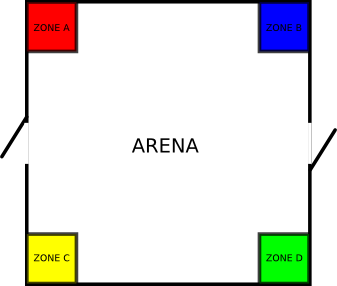
\includegraphics[keepaspectratio, scale =1]{../arena/arenagame2.png}
\caption{\small{\emph{The General Arena Layout}}}
\label {fig:arena}
\end {center}
\end {figure}
